\documentclass[12pt, letterpaper]{report}

\usepackage[utf8]{inputenc}
\usepackage{amsmath}
\usepackage{amsthm}
\usepackage{amsfonts}
\usepackage{amssymb}
\usepackage{enumerate}
\usepackage{graphicx}
\usepackage{mdframed}
\usepackage{multicol}
\usepackage{verbatim}
\usepackage{tikz}
\usepackage[margin = .8in]{geometry}
\linespread{1.2}
\usepackage{centernot}
\usepackage{float}
\usepackage{array}
\newcolumntype{C}[1]{>{\centering\arraybackslash}m{#1}}

\usepackage{xcolor}
\pagecolor[rgb]{0,0,0}
\color[rgb]{0.8,0.8,0.8}

\makeatletter
\renewcommand\thesubsection{%
  \thesection.\number\numexpr\value{subsection}-1\relax
}
\makeatother

\usepackage{fancyhdr}
\setlength{\headheight}{15pt}
\pagestyle{fancy}
\lhead{CMPT 477}
\chead{Mark Pepaj}
\rhead{\today}
\cfoot{Page \thepage}
\renewcommand{\footrulewidth}{0.4pt}% default is 0pt

\renewcommand{\thesubsection}{\small{\alph{subsection})}}

\begin{document}
    {\centering\large\textbf{Project 5}\par}
    \section*{Problem One}
    \textbf{Source Image:} Lena\_Y.tif
    \subsection{}
    \begin{figure}[htbp]
            \centering
            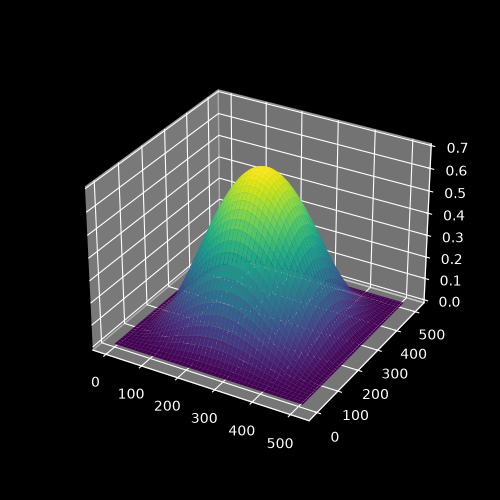
\includegraphics[width=0.5\textwidth]{images/smart_mean.png}
            \caption{Power Spectrum of Smart Mean Filter}
            \label{fig:smart_mean_filter}
        \end{figure}
    \subsection{}
    An analysis of the top left quarter of the image's Fourier power spectrum (x: 0-128, y: 0-128) shows that the first occurrence of a coefficient whose value is less than $0.1 \times 10^{-5}$ is at index (126, 127).
    This means that frequencies greater than or equal to 128 will be suppressed significantly.
    \subsection{}
    The image is $512 \times 512$ and the 2-D frequency at which the power spectrum coefficients started to become very small was 128. According to the Nyquist Sampling Theorem, frequencies of size 512/4 are responsible for details whose size are $2 \times 2$ pixels big. And since $512/128 = 4$, this means that details whose sizes are $2 \times 2$ pixels or smaller, will be suppressed or lost.
    \subsection{}
    \setcounter{subsection}{0}
        \begin{table}[htbp]
            \centering
            \begin{tabular}{|c|c|c|}
                \cline{1-3}
                \multicolumn{3}{|c|}{Spatial Domain Filtering of Gaussian Noise $(0.1\sigma)$}\\
                \cline{1-3}
                Clean Image & Noisy Image  & Filtered Image\\
                \hline
                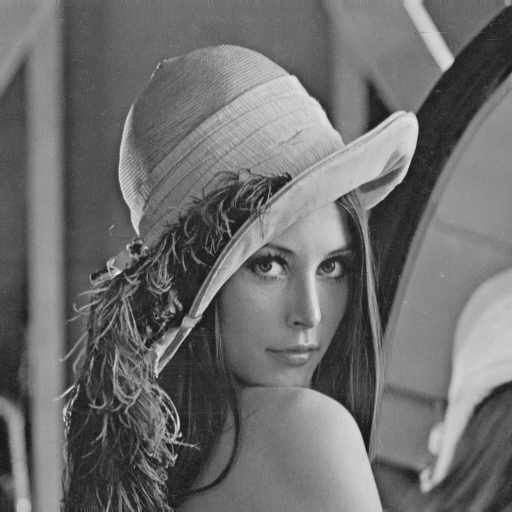
\includegraphics[width=0.3\textwidth]{images/Lena_Y.png} &  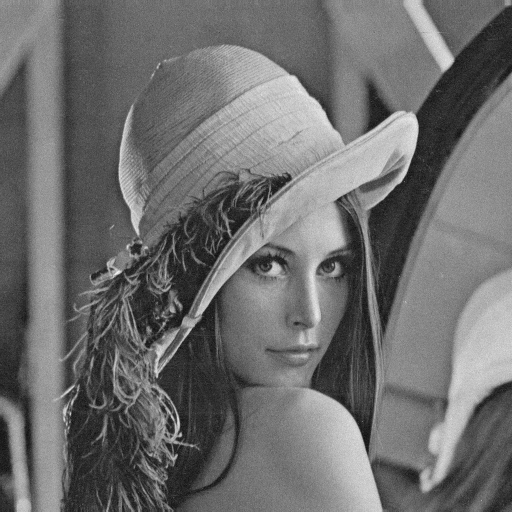
\includegraphics[width=0.3\textwidth]{images/noisy_Lena_Y.png} & 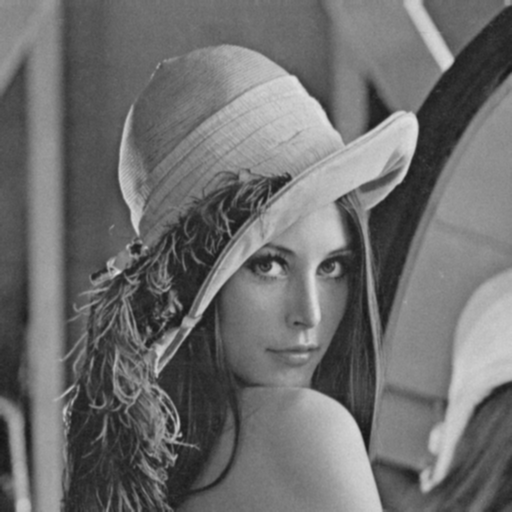
\includegraphics[width=0.3\textwidth]{images/spatial_filtered_Lena_Y.png}\\
                \hline
                                                                             & \textbf{PSNR} $34.9695$ & \textbf{PSNR:} $34.3871$\\
                \hline
            \end{tabular}
        \end{table}
        \begin{table}[htbp]
            \centering
            \begin{tabular}{|c|c|c|}
                \cline{1-3}
                \multicolumn{3}{|c|}{Frequency Domain Filtering of Gaussian Noise $(0.1\sigma)$}\\
                \cline{1-3}
                Clean Image & Noisy Image  & Filtered Image\\
                \hline
                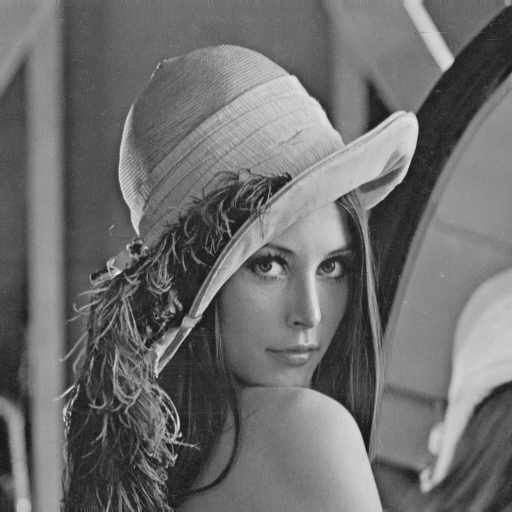
\includegraphics[width=0.3\textwidth]{images/Lena_Y.png} &  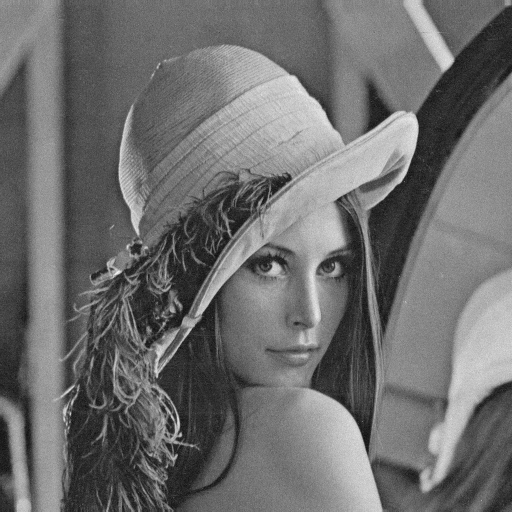
\includegraphics[width=0.3\textwidth]{images/noisy_Lena_Y.png} & 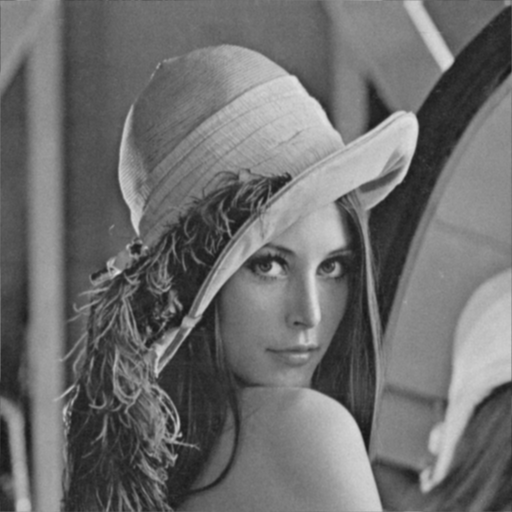
\includegraphics[width=0.3\textwidth]{images/frequency_filtered_Lena_Y.png}\\
                \hline
                                                                             & \textbf{PSNR} $34.9695$ & \textbf{PSNR:} $34.0534$\\
                \hline
            \end{tabular}
        \end{table}
        The above tables display the performance of the smart mean filter when tested on an image artificially corrupted with Gaussian noise with parameter $0.1\sigma$.
        The first table shows the results from filtering the image in the spatial domain.
        The PSNR drops slightly after filtering due to the smart mean filter removing some details from the image.
        Since the $\sigma$ is small, the image is corrupted with a very light noise and the filter is likely to strong for such light noise.

        The second table shows the results from filtering the image in the frequency domain.
        Part b) shows that frequencies higher than 256 are suppressed.
        This is reflected in the results of filtering the image in the frequency domain.
        The table shows that the image filtered in the frequency domain has a lower PSNR than the image filtered in the spatial domain. 
        This is likely due to the filter suppressing high frequencies in the image, which are responsible for small details.
        Moreover, similar to the filter in the spatial domain, the filter in the frequency domain is likely too strong for the light noise in the corrupted image.
    \section*{Problem Two}
    \textbf{Source Image:} Lena\_Y.tif
    \subsection{}
    \begin{figure}[H]
            \centering
            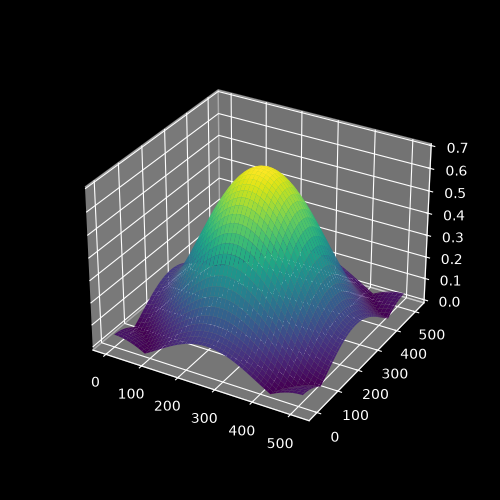
\includegraphics[width=0.5\textwidth]{images/improved_smart_mean.png}
            \caption{Power Spectrum of Improved Smart Mean Filter}
            \label{fig:improved_smart_mean_filter}
        \end{figure}
    \subsection{}
    ***An analysis of the top left quarter of the image's Fourier power spectrum (x: 0-128, y: 0-128) shows that the first occurrence of a coefficient whose value is less than $0.1 \times 10^{-5}$ is at index (126, 127).
    This means that frequencies greater than or equal to 128 will be suppressed significantly.
    \subsection{}
    ***The image is $512 \times 512$ and the 2-D frequency at which the power spectrum coefficients started to become very small was 128. According to the Nyquist Sampling Theorem, frequencies of size 512/4 are responsible for details whose size are $2 \times 2$ pixels big. And since $512/128 = 4$, this means that details whose sizes are $2 \times 2$ pixels or smaller, will be suppressed or lost.
    \subsection{}
        \begin{table}[H]
            \centering
            \begin{tabular}{|c|c|c|}
                \cline{1-3}
                \multicolumn{3}{|c|}{Spatial Domain Filtering of Gaussian Noise $(0.1\sigma)$}\\
                \cline{1-3}
                Clean Image & Noisy Image  & Filtered Image\\
                \hline
                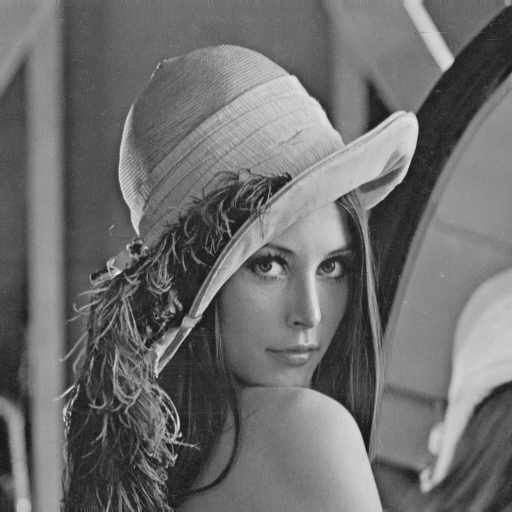
\includegraphics[width=0.3\textwidth]{images/Lena_Y.png} &  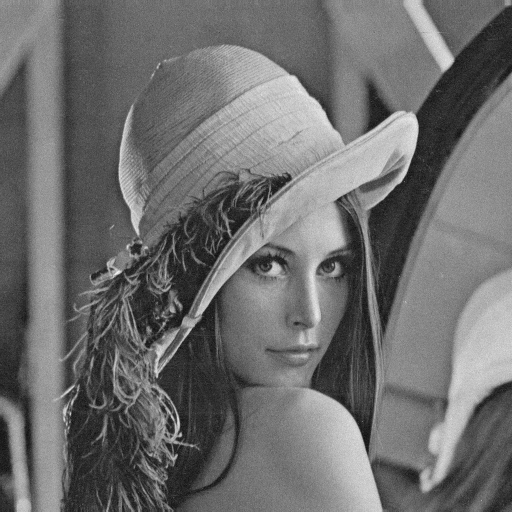
\includegraphics[width=0.3\textwidth]{images/noisy_Lena_Y.png} & 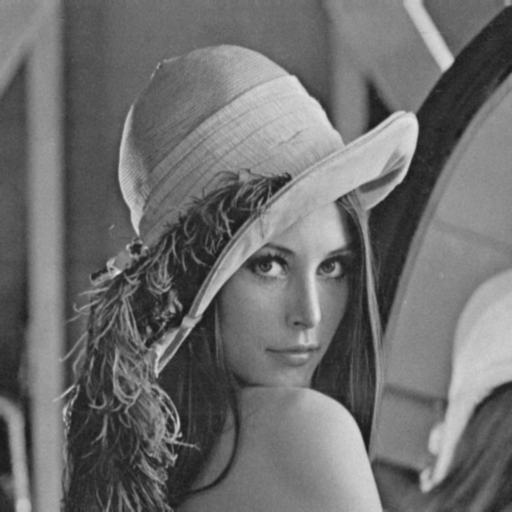
\includegraphics[width=0.3\textwidth]{images/improved_spatial_filtered_Lena_Y.png}\\
                \hline
                                                                             & \textbf{PSNR} $34.9855$ & \textbf{PSNR:} $35.0219$\\
                \hline
            \end{tabular}
        \end{table}
        \begin{table}[H]
            \centering
            \begin{tabular}{|c|c|c|}
                \cline{1-3}
                \multicolumn{3}{|c|}{Frequency Domain Filtering of Gaussian Noise $(0.1\sigma)$}\\
                \cline{1-3}
                Clean Image & Noisy Image  & Filtered Image\\
                \hline
                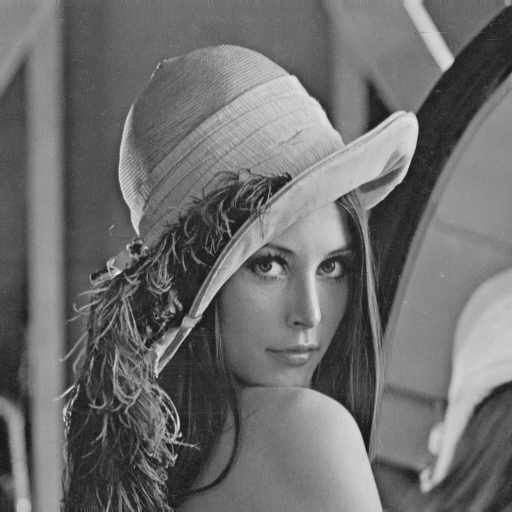
\includegraphics[width=0.3\textwidth]{images/Lena_Y.png} &  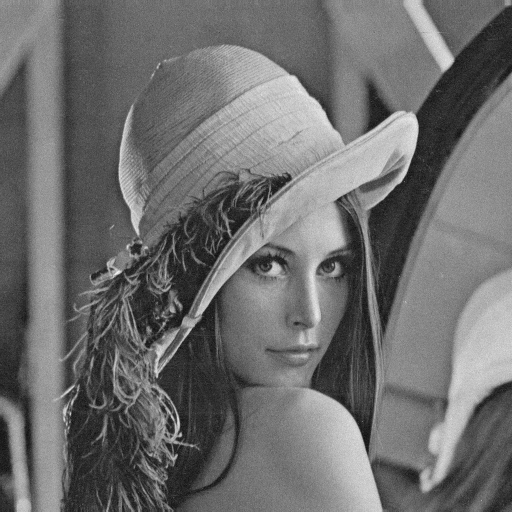
\includegraphics[width=0.3\textwidth]{images/noisy_Lena_Y.png} & 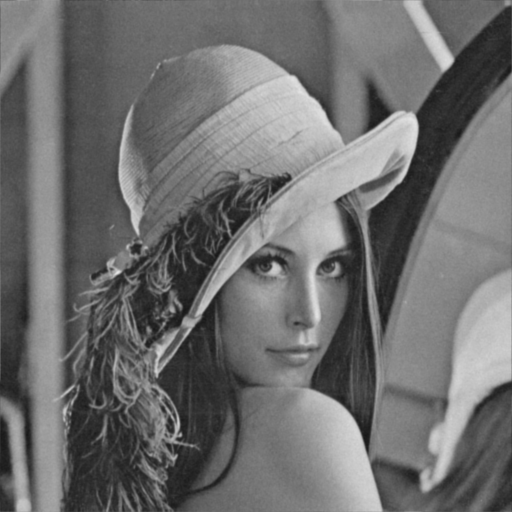
\includegraphics[width=0.3\textwidth]{images/improved_frequency_filtered_Lena_Y.png}\\
                \hline
                                                                             & \textbf{PSNR} $34.9855$ & \textbf{PSNR:} $34.7270$\\
                \hline
            \end{tabular}
        \end{table}
        The above tables display the performance of the smart mean filter when tested on an image artificially corrupted with Gaussian noise with parameter $0.1\sigma$.
        The first table shows the results from filtering the image in the spatial domain.
        Unlike the image filtered with the smart mean filter, the image filtered with the improved filter has a PSNR slightly higher than the PSNR of the corrupted image.

        The second table shows the results from filtering the image in the frequency domain. 
        The improved smart mean filter shows better results than the smart mean filter, while the PSNR of the image filtered in the frequency domain still falls behind the image filtered in the spatial domain.
        Again, this is likely due to the filter suppressing high frequencies, which correspond to small details in the image.
\end{document}
